\documentclass[tikz,border=10pt]{standalone}
\usetikzlibrary{calc}
\begin{document}
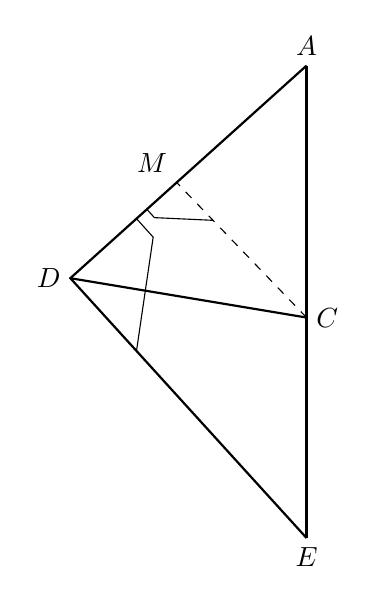
\begin{tikzpicture}
  \coordinate (A) at (3,3);
  \coordinate (D) at (0,0.3);
  \coordinate (E) at (3,-3);
  \coordinate (C) at (3,-0.2);
  \coordinate (M) at ($(A)!0.55!(D)$);

  \draw[thick] (A) -- (E);
  \draw[thick] (A) -- (D) -- (E);
  \draw[thick] (D) -- (C);
  \draw[dashed] (C) -- (M);

  % right-angle mark at D (between DA and DE)
  \draw ($(D)!0.28!(A)$) -- ($($(D)!0.28!(A)$)!0.28!90:(D)$) -- ($(D)!0.28!(E)$);

  % right-angle mark at M (between MC and MD)
  \draw ($(M)!0.28!(D)$) -- ($($(M)!0.28!(D)$)!0.28!-90:(M)$) -- ($(M)!0.28!(C)$);

  \node[above] at (A) {$A$};
  \node[left] at (D) {$D$};
  \node[below] at (E) {$E$};
  \node[right] at (C) {$C$};
  \node[above left] at (M) {$M$};
\end{tikzpicture}
\end{document}
